\section{Communication entre Telco et Commando}

\subsection{Décomposition des classes de communication}
\begin{figure}[H] 
    \centering
    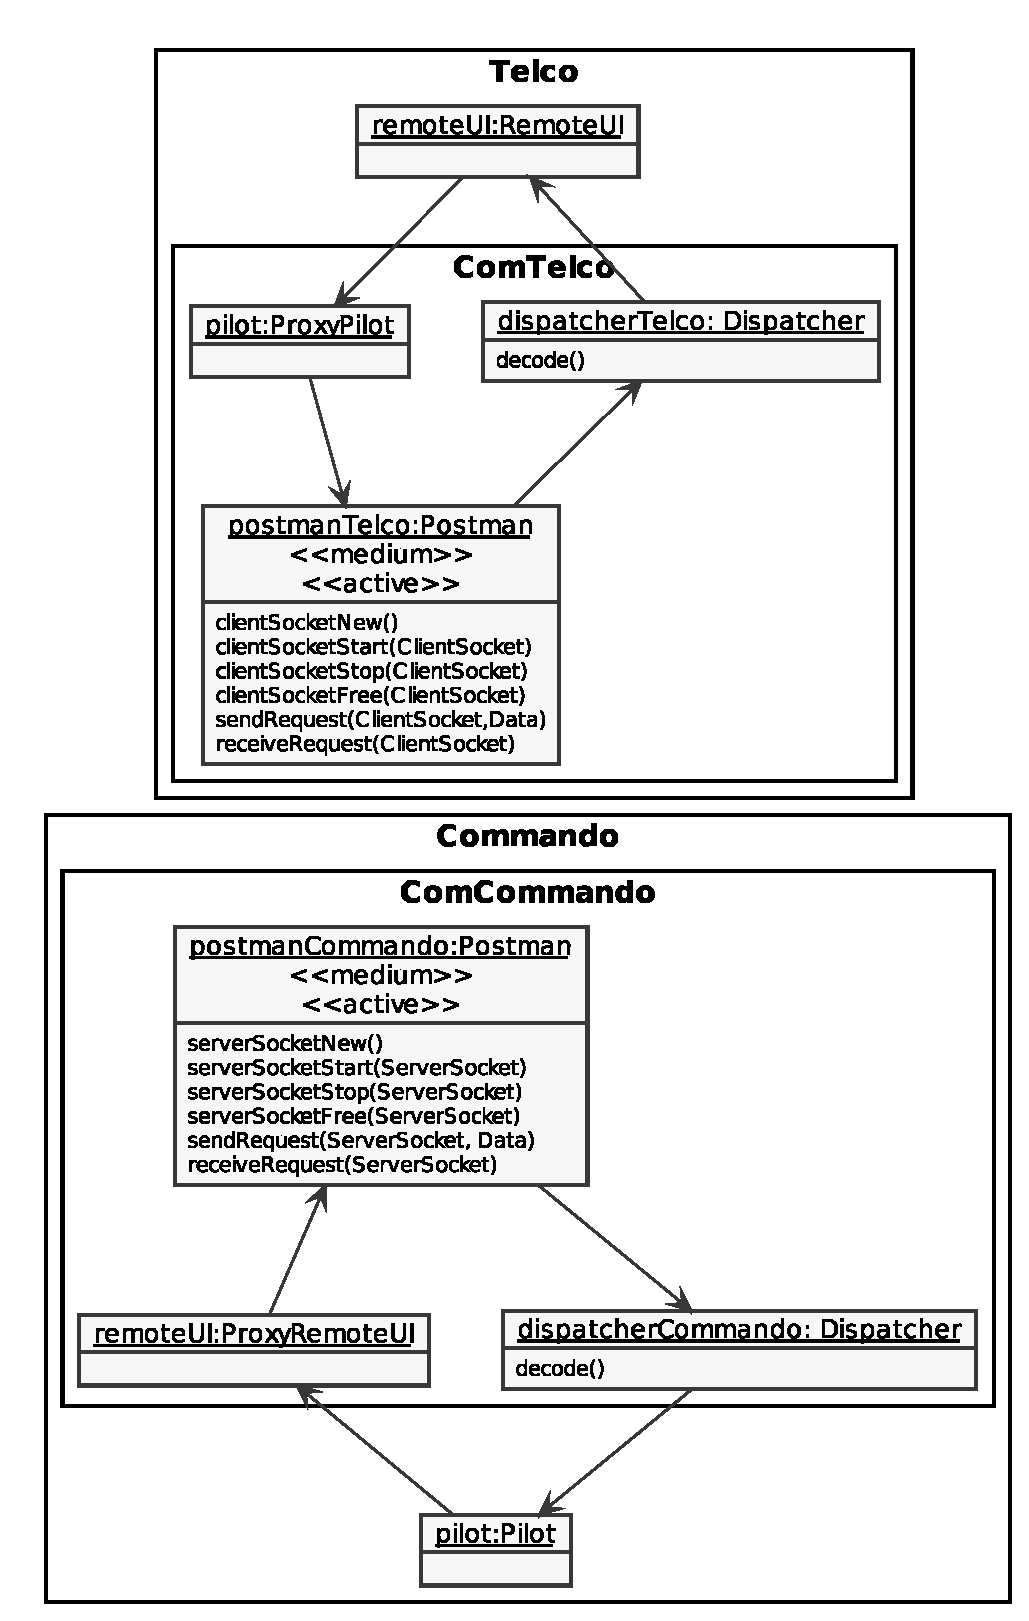
\includegraphics[width=0.8\textwidth]{img/diagrammeCommunication.eps}
    \caption{Diagramme de la communication entre Commando et Telco}
\end{figure}

\subsection{Protocole de communication}

La communication entre Telco et Commando se fera par socket, via des requêtes. Cette requête prendra la 
forme d’une chaîne de caractères qui contiendra plus ou moins d’informations selon la requète. 
\\

\paragraph{De Telco vers Commando\\ \\}

Telco doit pouvoir envoyer :
\begin{itemize}
    \item une demande d'arret d'urgence,
    \item une demande mouvement,
    \item une demande de la liste d'evenements,
    \item une demande du nombre d'evenements.
\end{itemize}
\medskip
On peut donc décomposer le message en deux parties :
\begin{itemize}
    \item l'id de la méthode appelé,
    \item les paramètres associés.
\end{itemize}

\medskip
\begin{table}[H]
    \centering
    \begin{tabular}{|
    >{\columncolor[HTML]{CE6301}}c |
    >{\columncolor[HTML]{009901}}c |}
    \hline
    {\color[HTML]{000000} \textbf{ID METHOD}} & {\color[HTML]{000000} \textbf{PARAMETRES}} \\ \hline
    \end{tabular}
    \caption{Forme de la requête de Telco vers Commando}
\end{table}

Association de la valeur à chaque méthode :
\medskip
\begin{table}[H]
    \centering
    \begin{tabular}{|m{6cm}|m{2cm}|}
        \hline
        \textbf{Méthodes} & \textbf{Valeur}  \\
        \hline
        demande de la liste d'evenements & 1 \\ \hline
        demande du nombre d'evenements & 2 \\ \hline
        demande mouvement & 3 \\ \hline
        demande d'arret d'urgence & 4 \\ \hline
    \end{tabular}
    \caption{Valeur associés aux différentes méthodes}
\end{table}

\medskip
Les paramètres sont passées sous forme d'une structure

\paragraph{De Telco vers Commando\\ \\}

Telco doit pouvoir envoyer :
\begin{itemize}
    \item réponse à une demande mouvement,
    \item réponse à une demande de la liste d'evenements,
    \item réponse à une demande du nombre d'evenements.
\end{itemize}
\medskip
On peut donc décomposer le message en deux parties :
\begin{itemize}
    \item l'id de la méthode appelé,
    \item les paramètres associés.
\end{itemize}

\medskip
\begin{table}[H]
    \centering
    \begin{tabular}{|
    >{\columncolor[HTML]{CE6301}}c |
    >{\columncolor[HTML]{009901}}c |}
    \hline
    {\color[HTML]{000000} \textbf{ID METHOD}} & {\color[HTML]{000000} \textbf{PARAMETRES}} \\ \hline
    \end{tabular}
    \caption{Forme de la requête de Commando vers Telco}
\end{table}

Association de la valeur à chaque méthode :
\medskip
\begin{table}[H]
    \centering
    \begin{tabular}{|m{8cm}|m{2cm}|}
        \hline
        \textbf{Méthodes} & \textbf{Valeur}  \\
        \hline
        réponse à demande de la liste d'evenements & 1 \\ \hline
        réponse à demande du nombre d'evenements & 2 \\ \hline
        réponse à demande mouvement & 3 \\ \hline
    \end{tabular}
    \caption{Valeur associés aux différentes méthodes}
\end{table}

\medskip
Les paramètres sont passées sous forme d'une structure
